%! suppress = LineBreak

\subsection{Insertion Sort}\label{subsec:insertion-sort-laufzeit}

In Abbildung~\ref{fig:isort} ist die Laufzeit mit zufälligen Zahlen und
aufsteigenden Zahlen zu sehen.
Der Plot ist eindeutig quadratisch.%TODO ausführen warum quadratisch
Die quadratische Laufzeit des Average-Case ist auch in
(Abbildung~\ref{fig:qsort-complexity-log}) als Log-Log Plot dargestellt.
\begin{figure}[hbt]
    \centering
    \caption{Insertion Sort}
    \subfloat[average case, worst case]{
    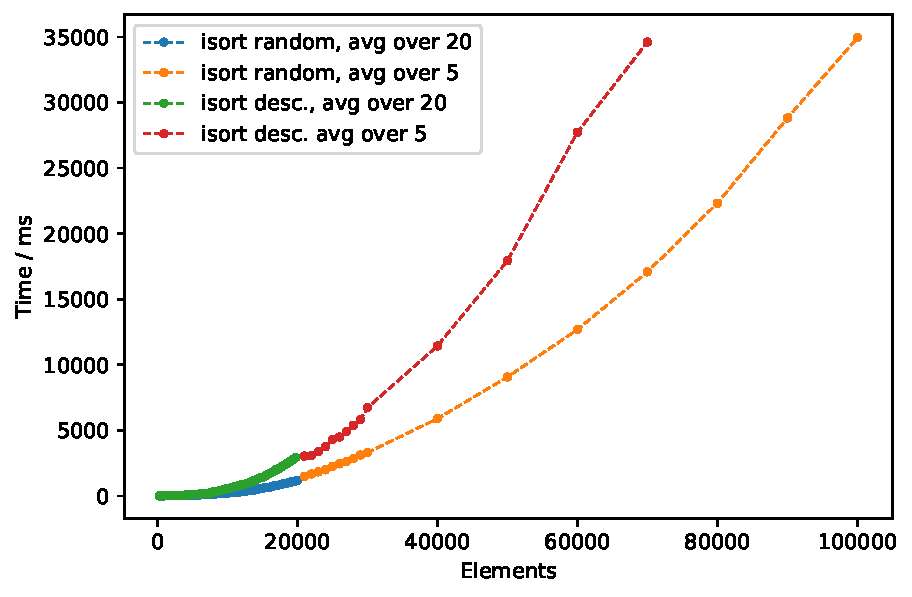
\includegraphics[width = 0.47\textwidth]
    {../out/isort.pdf}\label{fig:isort} }
    \hfill
    \subfloat[best case]{
    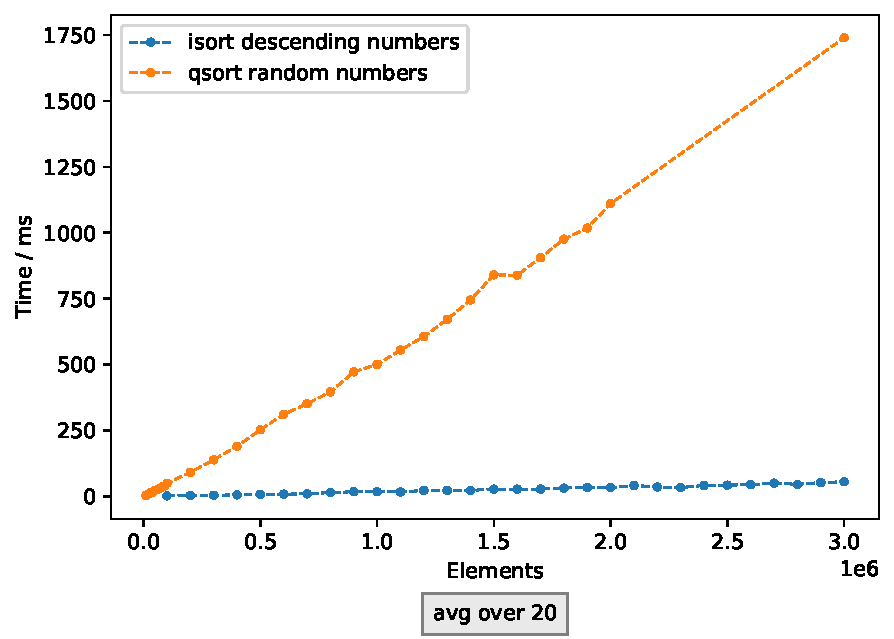
\includegraphics[width = 0.47\textwidth]
    {../out/isortBest.pdf}\label{fig:isort-best} }
\end{figure}

Der Best-Case ist in Abbildung~\ref{fig:isort-best} dargestellt.
Dieser tritt auf, wenn die Liste absteigend sortiert ist.
Dies lässt sich an der Erlang Implementation erklären, da bei absteigenden
Zahlen mit der \textit{insertToList()} Methode jeweils kleinere Zahlen in den
sortieren Abschnitt eingefügt werden.
Diese Operation hat eine Komplexität von \(\Theta(1)\), da die kleinere Zahl
der Liste vorangestellt wird.
Somit ergibt sich bei absteigenden Zahlen eine Gesamtkomplexität von
\(\Theta(n)\), da dieser diese Methode für alle Elemente der Liste ein Mal
ausgeführt wird.

Bei aufsteigenden Zahlen muss die \textit{insertToList()} Methode hingegen
jeweils bis zum Ende des sortieren Abschnitts laufen, da die Elemente jeweils
größer werden, wodurch eine Gesamtkomplexität von \(\Theta (n^2)\) entsteht.

Zusammenfassen haben wir also festgestellt, dass sich die Laufzeit unserer
Implementation von Insertion Sort durch \(O(n^2)\) und \(\Omega(n)\)
beschreiben lässt, was unseren Erwartungen entspricht.
\subsection{Quick Sort}\label{subsec:quick-sort-laufzeit}

\subsubsection{Pivot Methoden}

\paragraph{Erste Implementation}
Bei der ersten Implementation vom Quicksort Algorithmus ist bei der
Verwendung der Pivot-Methoden \(right\) und \(median\)  eine deutlich längere
Laufzeit aufgefallen (siehe Abbildung~\ref{fig:qsort-first-impl}).
Gleichzeit ist die Laufzeit von der \(middle\) Pivot Methode besser, obwohl
die Erwartung dieser schlechter ist:
Diese muss eineinhalb mal -- einmal zum Finden der Länge \(l\) komplett, danach
bis zum \(l/2\) Element -- durchlaufen werden.
Die Pivot Methode \(right\) muss nur einmal bis zum Ende der Liste laufen.

\begin{figure}[hbt]
    \caption{Vergleich der Pivot Methoden -- erste Implementation}
    \centering
    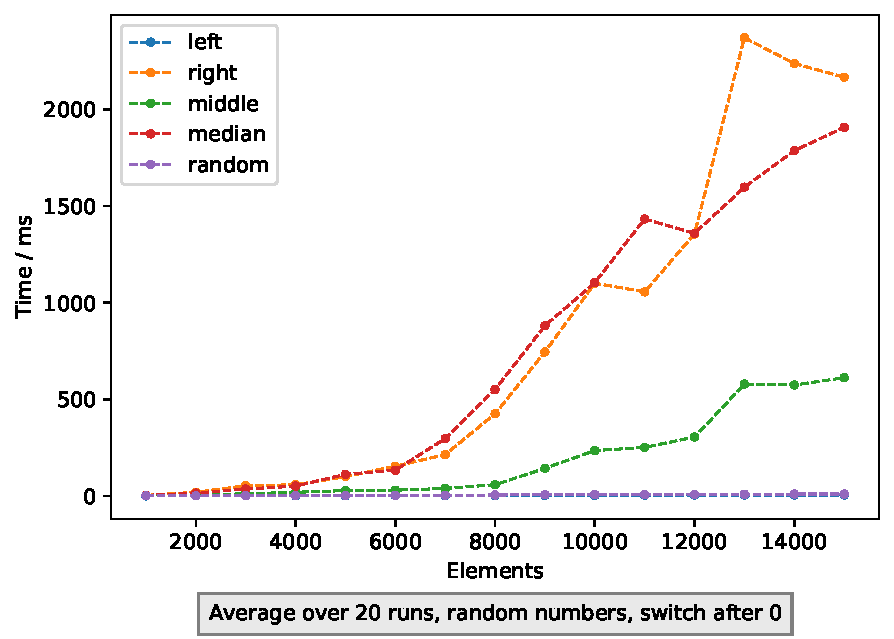
\includegraphics[width = 8cm]
    {../out/pivotMethods_Implementation1.pdf}\label{fig:qsort-first-impl}
\end{figure}

Unsere erste Vermutung war, dass unsere Methoden, die in einem
Durchlauf die Länge und gleichzeitig dass Pivot-Element ermitteln dafür
verantwortlich sein könnten.
In der Methoden zum Finden des letzten Elementes, die auch von der median
Pivot Methode verwendet wird, benutzten wir Pattern Matching, um zwischen dem
Letzten und vorletztem Element zu unterscheiden.
Dabei muss allerdings jeweils vorausgeschaut werden, was die schlechte
Performance erklären könnte.

Somit die Vermutung, dass man die Performance verbessern kann, indem man
zunächst die Länge der Liste ermittelt und anschließend diese zum Finden des
n-ten Elements ein zweites mal durchläuft.

\paragraph{Zweite Implementation}

In der zweiten Implementation wurden die Ermittlung des Pivots und das Finden
der Länge der Liste getrennt.
Das letzte Elements wurde nun ermittelt, indem zunächst
die Länge \(l\) der Liste berechnet, anschließend mithilfe dieser zum
\(l-1\) -ten Element gelaufen wird.
\begin{figure}[hbt]
    \centering
    \caption{Zweite Implementation vs. erste Implementation}
    \subfloat[median]{
    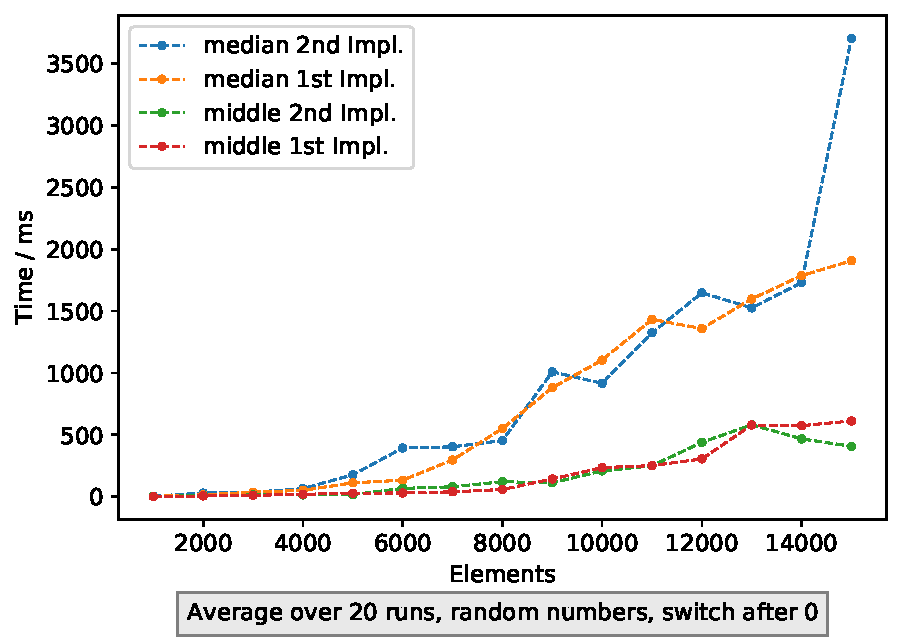
\includegraphics[width = 0.47\textwidth]
    {../out/pivotMethods_Implementation2b.pdf}\label{fig:qsort-impl2b} }
    \hfill
    \subfloat[right]{
    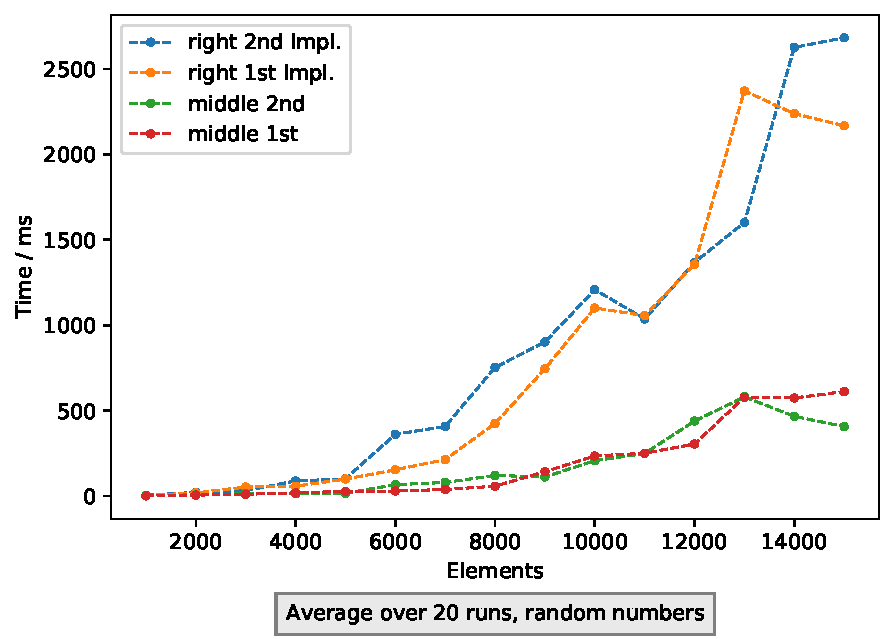
\includegraphics[width = 0.47\textwidth]
    {../out/pivotMethods_Implementation2a.pdf}\label{fig:qsort-impl2a} }
\end{figure}


In Abbildung~\ref{fig:qsort-impl2b} und~\ref{fig:qsort-impl2a} sind jeweils die
Ergebnisse der Laufzeitmessung der zweiten Implementation von \(median\) und
\(right\) zu sehen.
Damit systematische Unterschiede zwischen den beiden Kompilationen
ausgeschlossen sind, ist zusätzlich die gleiche Implementation, von \(middle\)
dargestellt.
Bei beiden überarbeiteten Implementationen ist keine Besserung der Laufzeit zu
erkennen, was darauf schließen lässt, dass das in der ersten Implementation
verwendete Pattern Matching nicht der Grund der schlechten Performance war.

\paragraph{Weitere Mögliche Ursachen}
Eine weitere Mögliche Ursache für die Ergebnisse ist der Fakt, das bei der
Methode zum finden des n-ten Elementes und des Restes
\textit{listGetNthAndRest()} die Erlang List Concatenation (\(++\)) verwendet
wird, und somit bei jedem Rekursionsschritt ein zusätzlicher Aufwand von
\(n\), wobei \(n\) die Anzahl der Elemente in der Subliste darstellt,
hinzukommt.
Dies würde auch erklären, warum \textit{middle} eine bessere Laufzeit
aufweist, da dabei nur ein zusätzlicher Aufwand von \(n/2\) halbe dazukommt.

\paragraph{Dritte Implementation}
In der dritten Implementation wurde die List Concatenation ersetzt.

\begin{figure}[hbt]
    \centering
    \caption{Dritte Implementation vs. erste Implementation}
    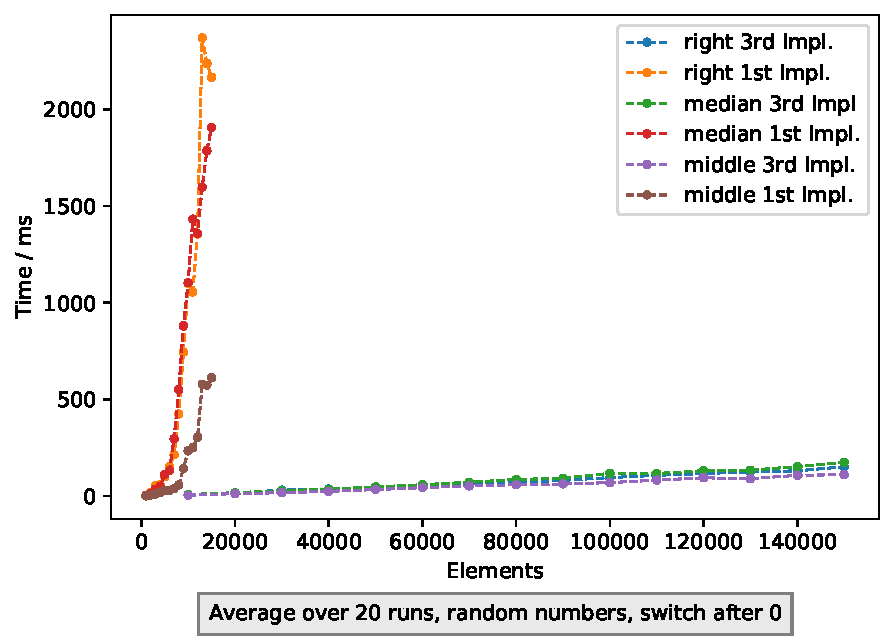
\includegraphics[width=8cm]
    {../out/pivotMethods_Implementation3.pdf}\label{fig:qsort-impl3}
\end{figure}

Wie in Abbildung~\ref{fig:qsort-impl3} zu sehen,
verbessert dies die Laufzeit dramatisch.
Die Laufzeit der Pivot Methode \textit{middle} hat sich auch verbessert, was
darauf zurückzuführen ist, dass diese ebenfalls die \textit{listGetNthAndRest
()} Methode verwendet.

\paragraph{Vergleich der Pivot Methoden}

In Abbildung~\ref{fig:qsort-impl3-2} ist die Laufzeit der Pivot Methoden der
dritten Implementation dargestellt.

\begin{figure}[hbt]
    \centering
    \caption{Vergleiche der Pivot Methoden -- Dritte Implementation}
    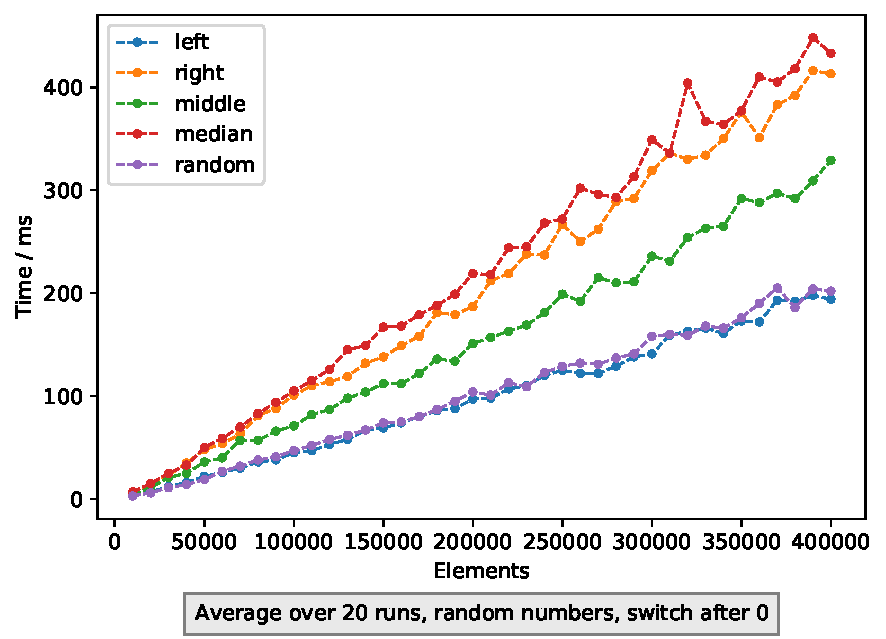
\includegraphics[width=8cm]
    {../out/pivotMethods.pdf}\label{fig:qsort-impl3-2}
\end{figure}

\FloatBarrier

\subsubsection{Switch Number}\label{subsubsec:switch-number}
Bei der Implementation des Quicksort-Algorithmus wird ein Parameter
\textit{switchnumber} übergeben, welches den Schwellenwert angibt, ab wann
von Quicksort auf Insertion Sort umgeschaltet werden soll.
In Abbildung~\ref{fig:qsort-switchPivot} sind
jeweils Laufzeitmessungen mit variierender \textit{switchnumber} zu sehen.
Es wird deutlich, dass im Average-Case die optimale \textit{switchnumber} bei
ca. 20--50 Elementen liegt.

In Abbildung~\ref{fig:qsort-switchWorst} ist die \textit{switchnumber} im
Worst-Case von Quicksort untersucht worden.
An den Daten zu absteigenden Zahlen befindet sich Insertion Sort im Best-Case
und hat somit eine Laufzeit von \(\Omega(N)\), dies erklärt, warum der
Verlauf mit zunehmender \textit{switchnumber} scheinbar gegen 0ms läuft.
(Zu Details zum Best-Case von Insertion Sort, siehe
Abbildung~\ref{fig:isort-best} in
Abschnitt~\ref{subsec:insertion-sort-laufzeit})

An den Daten zu aufsteigenden Zahlen befindet sich Insertion Sort im
Average-Case und hat eine Komplexität von \(O(n^2)\).
Da Quicksort im Worst-Case ebenfalls eine Komplexität von \(O(n^2)\)
aufweist, wird hierdurch verdeutlicht, dass der Aufwand pro Iteration, also
der Faktor vor dem \(n\), bei Insertion Sort geringer ist als bei Quicksort.

%TODO

\begin{figure}[hbt]
    \centering
    \caption{Vergleich der Switch Number}
    \subfloat[Average Case]{
    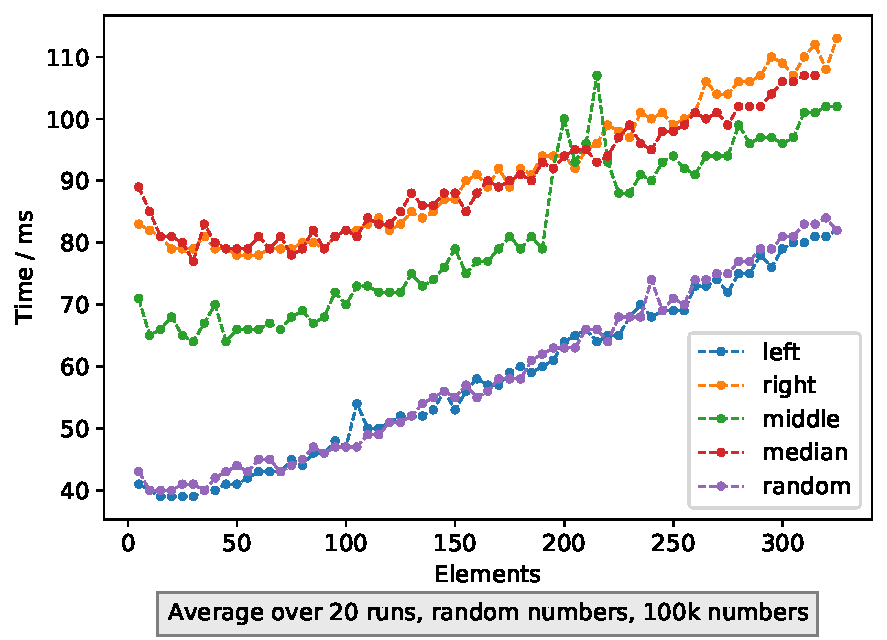
\includegraphics[width = 0.47\textwidth]
    {../out/switchPivot.pdf}\label{fig:qsort-switchPivot} }
    \subfloat[Worst Case]{
    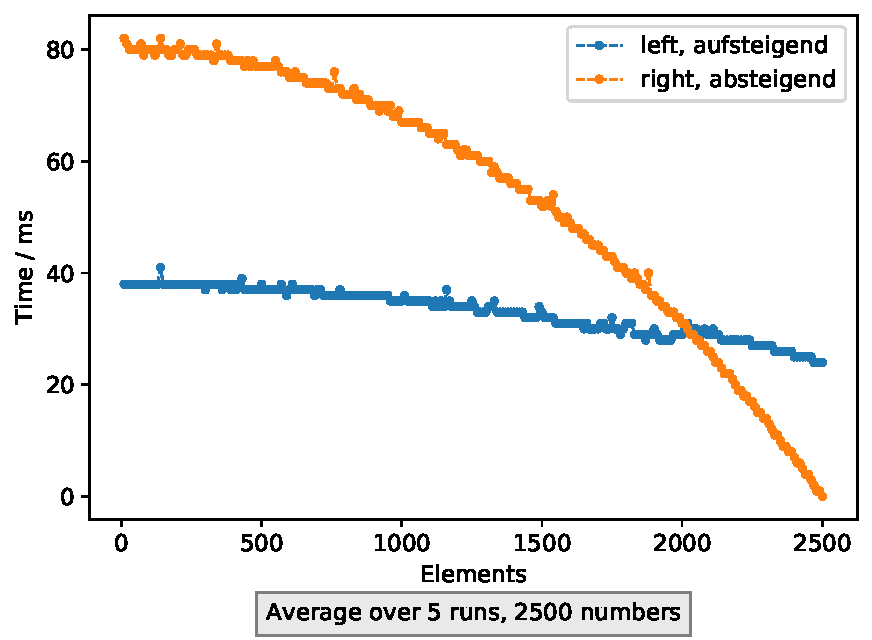
\includegraphics[width = 0.47\textwidth]
    {../out/switchWorstCase.pdf}\label{fig:qsort-switchWorst} }
\end{figure}

\subsubsection{Best Case}\label{subsubsec:qsort-best-case}

An dem linearen Plot (Abbildung~\ref{fig:qsort-complexity})
ist kaum zu erkennen, ob eine lineare oder
über-logarithmische Komplexität vorliegt.
Wir haben uns erhofft, dies mithilfe eines Log-Log Plots
(Abbildung~\ref{fig:qsort-complexity-log}) genauer zu untersuchen.
Auf solchem ist Anhand der Steigung des Graphen der Exponent zu erkennen.
Somit müsste die Steigung unserer Messkurve zwischen den beiden Funktionen
\(f(x)=x\) und \(f(x)=x^2\) liegen, falls diese über-logarithmisch ist.

Leider lässt sich auch auf diesem nicht zwischen dem linearem und, nach
unserer Erwartung, über-logarithmischen Messkurve unterscheiden.

\begin{figure}[hbt]
    \centering
    \caption{Best Case}
    \subfloat[Linearer Plot]{
    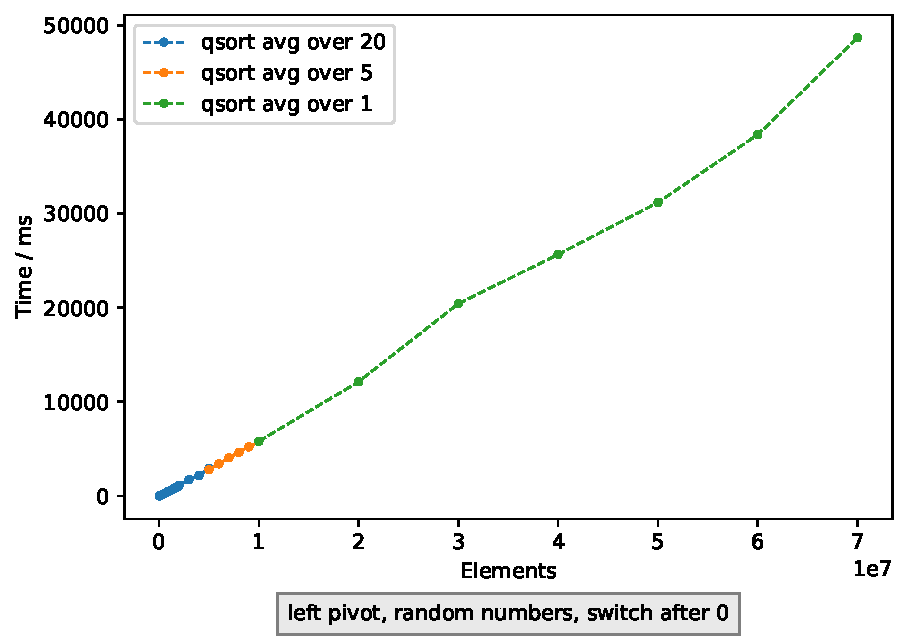
\includegraphics[width = 0.47\textwidth]
    {../out/complexity.pdf}\label{fig:qsort-complexity} }
    \subfloat[Log-Log Plot]{
    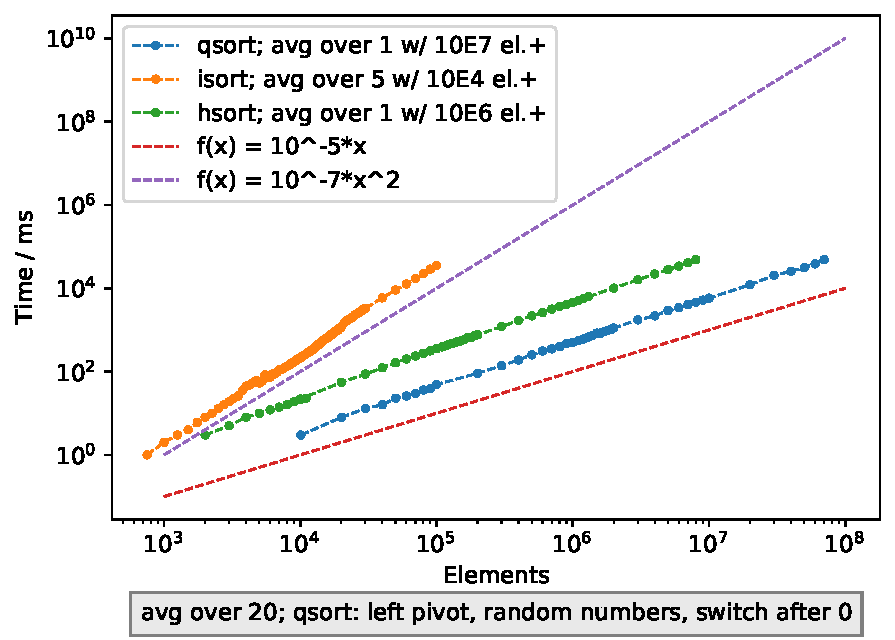
\includegraphics[width = 0.47\textwidth]
    {../out/complexityLog.pdf}\label{fig:qsort-complexity-log} }
\end{figure}

\subsubsection{Worst Case}\label{subsubsec:worst-case}
Die Laufzeit zum Worst Case wurde kurz im
Abschnitt~\ref{subsubsec:switch-number} besprochen.
Aus zeitlichen Gründen werden wir nicht weiter darauf eingehen.

% TODO avg kann so niedrig sein weil aufsteigend, heisst keine varianz der
%zahlen
% hier eigentlich vergleich von isort und qsort
% right, absteigend geht auf null, da die isort laufzeit von sortierten
% listen thetha(n) (?) ist

\FloatBarrier

\subsection{Heap Sort}\label{subsec:heap-sort-laufzeit}
